% command to make sure colorboxes don't create whitespace between code lines
\fboxsep=.6pt

% default settings for listings
\lstset{style=python}

\title[Daten Vorhersagen]{Daten Vorhersagen}

\subtitle{Korrelation \& Kausalität}

\author[Wendl, Cyril] % (optional)
{Cyril Wendl}

\institute[KLW] % (optional)
{
    Fachschaft Informatik\\
    Kantonsschule im Lee
}

\date[\today] % (optional)

\logo{
\includegraphics[width=2cm]{Logos/LeeLogo}}

\titlegraphic{\vspace{-.7cm}\includegraphics[width=\textwidth]{"Grundlagen_Info/06_Datenbanken/Figures/title-emojis"}}

\frame{\titlepage}

\begin{frame}{Maschinelles Lernen}
    \begin{figure}[H]
        \only<1->{\centering
\includegraphics[width=0.26\pagewidth]{"Grundlagen_Info/10_Aus_Daten_Lernen/Figures/intro_spam.jpg"}}
        \only<2->{\centering
\includegraphics[width=0.26\pagewidth]{"Grundlagen_Info/10_Aus_Daten_Lernen/Figures/intro_YT.jpg"}}
        \only<3->{\centering
\includegraphics[width=0.26\pagewidth]{"Grundlagen_Info/10_Aus_Daten_Lernen/Figures/intro_scan.jpg"}}
        % \only<4->{\centering
\includegraphics[width=0.3\pagewidth]{"Grundlagen_Info/10_Aus_Daten_Lernen/Figures/intro_recommendation.jpg"}}
    \end{figure}
\end{frame}

\begin{frame}{Haarlänge und Notenschnitt}
    \begin{adjustwidth}{-1em}{-1em}
        \begin{center}
            Am Anfang steht häufig ein Vergleich zweier \\
            Variablen (= Datenreihen), z.B.:
        \end{center}
        \begin{columns}
            \column{0.9\textwidth}
            \begin{figure}[H]
                \centering
                \includegraphics[width=\linewidth]{"Grundlagen_Info/10_Aus_Daten_Lernen/Figures/haarlange_vs_notenschnitt"}
            \end{figure}
            \column{0.23\textwidth}
            \only<2->{Positive \textbf{Korrelation}: \\
                $\uparrow$ Haarlänge \\
                $\uparrow$ Notenschnitt\\[1cm]
            }
            \only<3->{aber gibt es auch eine \textbf{Kausalität}?}
        \end{columns}
    \end{adjustwidth}
\end{frame}

\begin{frame}[fragile]{Ziele der heutigen Lektion}
    \begin{itemize}[<+->]
        \item \faSquare{} Ich kann beschreiben, was \textbf{Korrelation} und \textbf{Kausalität} sind.
        \item \faSquare{} Ich kann begründen, welche Art der Beeinflussung zwischen zwei Variablen vorliegt.
        \item \faSquare{} Ich wende bei der Interpretation von Datenreihen Vorsicht an, bevor ich Aussagen über Ursache und Wirkung treffe.
        \item \faSquare{} Ich kann die Zahl \( Z \) berechnen und interpretieren.
    \end{itemize}
\end{frame}

\begin{frame}{Definition: Kausalität}
    \begin{mydefinition}[Kausalität]
    \begin{itemize}[<+->]
        \item \textbf{Ursache-Wirkung}-Beziehung zwischen zwei Variablen A und B.
        \item Ursprung des Begriffs: lat. \textit{causa} = Ursache
        \item Bedarf eines Nachweises (z.B. Experimente oder statistische Analysen).
        \item Verschiedenen Arten von Kausalität existieren.
    \end{itemize}
    \end{mydefinition}
\end{frame}

\begin{frame}{Arten von Kausalität: Koinzidenz (=Nicht-Kausalität)}
    \begin{center}
        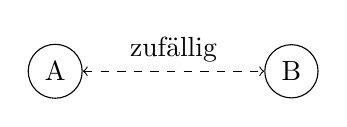
\begin{tikzpicture}
            \node[circle, draw] (A) at (0,0) {A};
            \node[circle, draw] (B) at (3,0) {B};
            \draw[<->, dashed] (A) -- (B) node[midway, above] {zufällig};
        \end{tikzpicture}
    \end{center}
    \only<2>{\begin{center}
            Beispiel: \textit{Im Zeitraum 2000-2009 sind in den USA sowohl der Pro-Kopf-Verbrauch von Mozzarella als auch die Anzahl Ingenieursabschlüsse angestiegen.}
        \end{center}}
\end{frame}

\begin{frame}{Arten von Kausalität: Zyklische Beeinflussung}
    \begin{center}
        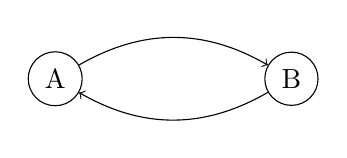
\begin{tikzpicture}
            \node[circle, draw] (A) at (0,0) {A};
            \node[circle, draw] (B) at (3,0) {B};
            \draw[->] (A) to[bend left] (B);
            \draw[->] (B) to[bend left] (A);
        \end{tikzpicture}
    \end{center}
    \only<2>{\begin{center}
            Beispiel: \textit{Schlafmangel führt zu mehr Stress, was wiederum zu mehr Schlafmangel führt.}
        \end{center}}
\end{frame}

\begin{frame}{Arten von Kausalität: Gemeinsamer Grund}
    \begin{center}
        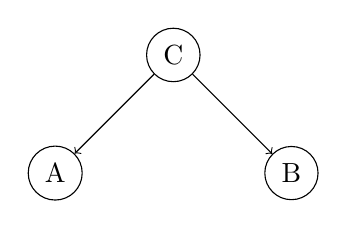
\begin{tikzpicture}
            \node[circle, draw] (C) at (1.5,1.5) {C};
            \node[circle, draw] (A) at (0,0) {A};
            \node[circle, draw] (B) at (3,0) {B};
            \draw[->] (C) -- (A);
            \draw[->] (C) -- (B);
        \end{tikzpicture}
    \end{center}
    \only<2>{\begin{center}
            Beispiel: \textit{Zwischen November und Januar steigen sowohl der Verkauf von Winterreifen als auch die Häufigkeit von Erkältungen an.}
        \end{center}}
\end{frame}

\begin{frame}{Arten von Kausalität: Indirekte Kausalität}
    \begin{center}
        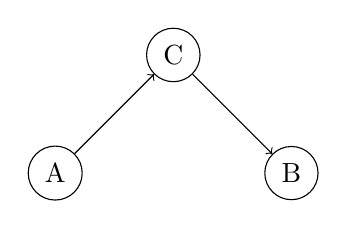
\begin{tikzpicture}
            \node[circle, draw] (A) at (0,0) {A};
            \node[circle, draw] (C) at (1.5,1.5) {C};
            \node[circle, draw] (B) at (3,0) {B};
            \draw[->] (A) -- (C);
            \draw[->] (C) -- (B);
        \end{tikzpicture}
    \end{center}
    \only<2>{\begin{center}
            Beispiel: \textit{Sport führt zu besserem Schlaf, was wiederum zu besseren Prüfungsergebnissen führt.}
        \end{center}}
\end{frame}

\begin{frame}{Arten von Kausalität: Direkte Kausalität}
    \begin{center}
        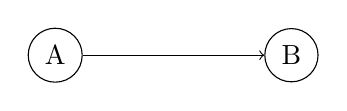
\begin{tikzpicture}
            \node[circle, draw] (A) at (0,0) {A};
            \node[circle, draw] (B) at (3,0) {B};
            \draw[->] (A) -- (B);
        \end{tikzpicture}
    \end{center}
    \only<2>{\begin{center}
            Beispiel: \textit{Mehr Video-Streams führen automatisch zu mehr Einnahmen für die Youtuberin.}
        \end{center}}
\end{frame}

\begin{frame}{Avocados und Maturaprüfungen}
    \begin{center}
        \enquote{In den letzten zehn Jahren hat der Konsum von Avocados in der Schweiz zugenommen. Im gleichen Jahrzehnt ist die Zahl bestandener Maturaprüfungen gestiegen.}
    \end{center}
    \begin{enumerate}
        \item \only<1>{Koinzidenz}\only<2>{\textbf{Koinzidenz}}
        \item Zyklische Beeinflussung
        \item Gemeinsamer Grund
        \item Indirekte Kausalität
        \item Direkte Kausalität
    \end{enumerate}
    \only<2>{\begin{center}
            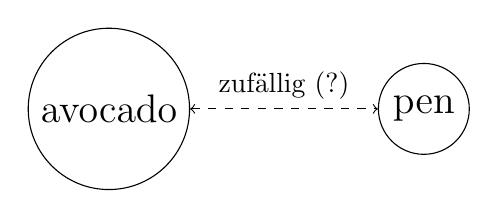
\begin{tikzpicture}
                \node[circle, draw] (A) at (0,0) {\Large\emoji{avocado}};
                \node[circle, draw] (B) at (4,0) {\Large\emoji{pen}};
                \draw[<->, dashed] (A) -- (B) node[midway, above] {zufällig (?)};
            \end{tikzpicture}
        \end{center}}
\end{frame}

\begin{frame}{Sonnenbrände und Glacé}
    \begin{center}
        \enquote{In den Sommermonaten nehmen sowohl die Anzahl Sonnenbrände wie auch der Verkauf von Glacé zu.}
    \end{center}
    \begin{enumerate}
        \item Koinzidenz
        \item Zyklische Beeinflussung
        \item \only<1>{Gemeinsamer Grund}\only<2>{\textbf{Gemeinsamer Grund}}
        \item Indirekte Kausalität
        \item Direkte Kausalität
    \end{enumerate}
    \only<2>{\begin{center}
            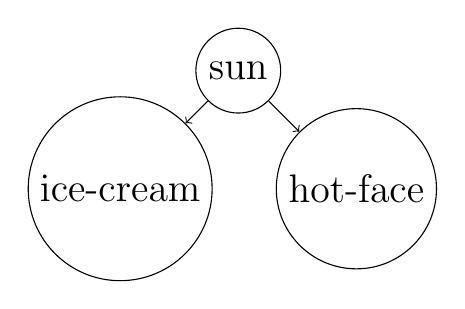
\begin{tikzpicture}
                \node[circle, draw] (C) at (1.5,1.5) {\Large\emoji{sun}};
                \node[circle, draw] (A) at (0,0) {\Large\emoji{ice-cream}};
                \node[circle, draw] (B) at (3,0) {\Large\emoji{hot-face}};
                \draw[->] (C) -- (A);
                \draw[->] (C) -- (B);
            \end{tikzpicture}
        \end{center}}
\end{frame}

\begin{frame}{Hunde und Übergewicht}
    \begin{center}
        \enquote{Eine Studie hat gezeigt, dass HunderbesitzerInnen weniger Risiko haben, übergewichtig zu werden.}
    \end{center}
    \begin{enumerate}
        \item Koinzidenz
        \item Zyklische Beeinflussung
        \item Gemeinsamer Grund
        \item \only<1>{Indirekte Kausalität}\only<2>{\textbf{Indirekte Kausalität}}
        \item Direkte Kausalität
    \end{enumerate}
    \only<2>{\begin{center}
            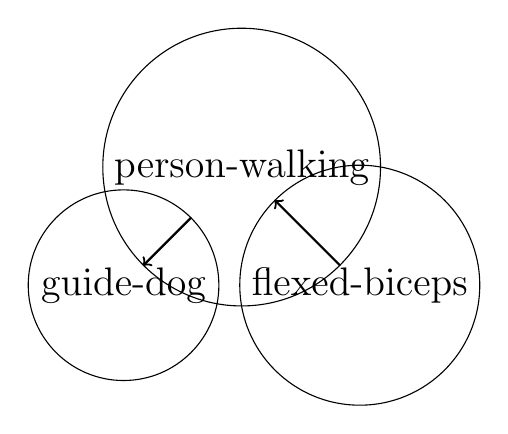
\begin{tikzpicture}
                \node[circle, draw, minimum size=1cm] (A) at (0,0) {\Large\emoji{guide-dog}};
                \node[circle, draw, minimum size=1cm] (C) at (1.5,1.5) {\Large\emoji{person-walking}};
                \node[circle, draw, minimum size=1cm] (B) at (3,0) {\Large\emoji{flexed-biceps}};
                \draw[->, thick] (A) -- (C);
                \draw[->, thick] (C) -- (B);
            \end{tikzpicture}
        \end{center}}
\end{frame}

\begin{frame}{Stress und Noten}
    \begin{center}
        \enquote{Eine Untersuchung von 1000 SchülerInnnen hat gezeigt, dass SchülerInnen, welche gestresster sind, schlechtere Noten erzielen.}
    \end{center}
    \begin{enumerate}
        \item Koinzidenz
        \item \only<1>{Zyklische Beeinflussung}\only<2>{\textbf{Zyklische Beeinflussung}}
        \item Gemeinsamer Grund
        \item Indirekte Kausalität
        \item Direkte Kausalität
    \end{enumerate}
    \only<2>{\begin{center}
            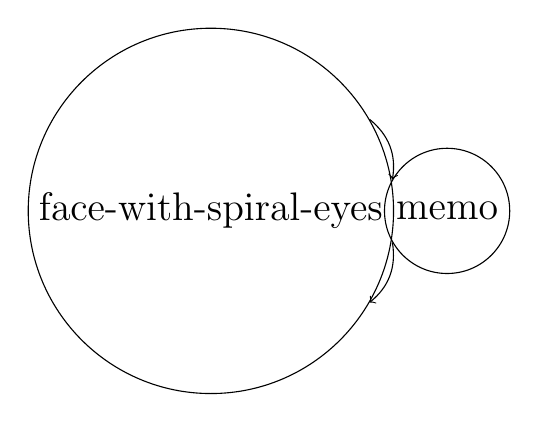
\begin{tikzpicture}
                \node[circle, draw] (A) at (0,0) {\Large\emoji{face-with-spiral-eyes}};
                \node[circle, draw] (B) at (3,0) {\Large\emoji{memo}};
                \draw[->] (A) to[bend left] (B);
                \draw[->] (B) to[bend left] (A);
            \end{tikzpicture}
        \end{center}}
\end{frame}

\begin{frame}{Definition: Korrelation}
    \begin{mydefinition}[Korrelation]
    \begin{itemize}[<+->]
        \item Statistische Beziehung zwischen zwei Variablen.\\
              Z.B.: $\uparrow$ \textit{Haarlänge}, $\uparrow$ \textit{Notenschnitt}
        \item Ursprung des Begriffs:
              \begin{itemize}
                  \item \textit{co(n)-} = \enquote{mit}.
                  \item \textit{relatio} = Beziehung.
              \end{itemize}
        \item Bedeutung: Gegenseitige Beziehung oder Wechselbeziehung (\emoji{arrows-counterclockwise}).
        \item Häufig als Zahl ausgedrückt (r, von -1 bis +1)
    \end{itemize}
    \end{mydefinition}
\end{frame}

\begin{frame}{Korrelations-Beispiele}
    \begin{figure}[H]
        \centering
        \foreach \corr in {
                -1, -0.8, 0, 0.8, 1
            } {\begin{subfigure}[t]{0.24\pagewidth}
                    \centering
                    \includegraphics[width=\linewidth]{"Grundlagen_Info/10_Aus_Daten_Lernen/Figures/correlation_\corr"}
                    \caption{r=\textbf{\corr}}
                \end{subfigure}
            }
        \only<2->{
            \begin{subfigure}[t]{0.24\pagewidth}
                \centering
                \includegraphics[width=\linewidth]{"Grundlagen_Info/10_Aus_Daten_Lernen/Figures/correl_ex_15"}
                \caption{r$\simeq$\textbf{0}}
            \end{subfigure}
        }
    \end{figure}
\end{frame}

\begin{frame}{Korrelations-Beispiele}
    \begin{figure}[H]
        \centering
        \only<1>{
\includegraphics[width=.75\pagewidth]{"Grundlagen_Info/10_Aus_Daten_Lernen/Figures/socialmedia_vs_zufriedenheit.pdf"}}
        \only<2>{
\includegraphics[width=.75\pagewidth]{"Grundlagen_Info/10_Aus_Daten_Lernen/Figures/haarlange_vs_notenschnitt.pdf"}}
        \only<3>{
\includegraphics[width=.75\pagewidth]{"Grundlagen_Info/10_Aus_Daten_Lernen/Figures/buecher_vs_schuhgroesse.pdf"}}
    \end{figure}
    $\rightarrow$ r-Wert? Positiv / negativ?
\end{frame}

\begin{frame}{Korrelations-Beispiel: Abweichung vom Mittelwert}
    \begin{adjustwidth}{-.5cm}{-.5cm}
        \begin{onlyenv}<1>
            \begin{figure}[H]
                \centering
                \includegraphics[width=.9\textwidth]{"Grundlagen_Info/10_Aus_Daten_Lernen/Figures/polizei_vs_kriminalitaet_correl"}
            \end{figure}
        \end{onlyenv}
        \begin{onlyenv}<2>
            \begin{figure}[H]
                \centering
                \includegraphics[width=.9\textwidth]{"Grundlagen_Info/10_Aus_Daten_Lernen/Figures/polizei_vs_kriminalitaet_correl_mean"}
            \end{figure}
        \end{onlyenv}
        \begin{onlyenv}<3->
            \begin{figure}[H]
                \centering
                \includegraphics[width=.9\textwidth]{"Grundlagen_Info/10_Aus_Daten_Lernen/Figures/polizei_vs_kriminalitaet_correl_norm"}
            \end{figure}
        \end{onlyenv}
        \only<2>{\textbf{1. Schritt:} Beide Mittelwerte berechnen ($\overline{x}$ und $\overline{y}$)}
        \only<3>{\textbf{2. Schritt:} Neue Werte $x'=x-\overline{x}$ und $y'=y-\overline{y}$ berechnen}
        \only<4->{\textbf{3. Schritt:} \(
            Z = x_1' \cdot y_1'\only<4>{+\dots} \only<5->{+ x_2' \cdot y_2'}\only<5>{+\dots} \only<6->{+ \dots + x_n' \cdot y_n'}
            \)}
    \end{adjustwidth}
\end{frame}

\begin{frame}[fragile]{Auftrag: Zu zweit}
    \begin{itemize}
        \item Auf Abschnitt \enquote{\textbf{Data Science}} auf Moodle gehen (zuoberst, nach \enquote{Allgemeine Informationen})
        \item Excel-Datei \enquote{\texttt{korrelation.xlsx}} herunterladen und öffnen
        \item Arbeitsblatt \enquote{\texttt{Beispiel}} genau anschauen $\rightarrow$ bereits gemacht, nichts ändern!
        \item Arbeitsblätter \enquote{\texttt{Aufgabe 1}} und \enquote{\texttt{Aufgabe 2}} lösen
        \item \challengebox{Viertes Arbeitsblatt lösen}
    \end{itemize}

    \begin{table}[H]
        \centering
        \begin{tabular}{l|l}
            \textbf{Excel-Befehl}   & \textbf{Bedeutung}             \\\midrule\midrule
            \verb|=MITTELWERT(...)| & Mittelwert berechnen           \\\midrule
            \verb|=SUMME(...)|      & Summe berechnen                \\\midrule
            \verb|=A1*B1|           & Zahlen multiplizieren          \\\midrule
            \verb|=$A$2|            & Referenz auf Zelle A2 fixieren \\
        \end{tabular}
    \end{table}
    \challengebox{Auftrag 1.6 und 1.7 im Skript}
\end{frame}

\begin{frame}{Berufserfahrung und Einladungswahrscheinlichkeit}
    \begin{columns}
        \column{0.7\textwidth}
        \begin{figure}[H]
            \centering
            \includegraphics[width=\linewidth]{"Grundlagen_Info/10_Aus_Daten_Lernen/Figures/berufserfahrung_vs_einladung"}
        \end{figure}
        \column{0.3\textwidth}
        Z=\textbf{44.66} \\$\rightarrow$ positive Korrelation.\\[.5cm]

        \only<2->{
            Kausalität?
            \begin{enumerate}
                \item Koinzidenz
                \item Zyklische Beeinflussung
                \item Gemeinsamer Grund
                \item Indirekte Kausalität
                \item \only<2>{Direkte Kausalität}\only<3>{\textbf{Direkte Kausalität?}}
            \end{enumerate}
        }
    \end{columns}
    \only<3>{Müsste wissenschaftlich untersucht werden...}
\end{frame}

\begin{frame}{Social-Media-Nutzung und Zufriedenheit}
    \begin{columns}
        \column{0.7\textwidth}
        \begin{figure}[H]
            \centering
            \includegraphics[width=\linewidth]{"Grundlagen_Info/10_Aus_Daten_Lernen/Figures/socialmedia_vs_zufriedenheit"}
        \end{figure}
        \column{0.3\textwidth}
        Z=\textbf{-30.13} \\$\rightarrow$ negative Korrelation.\\[.5cm]

        \only<2->{
            Kausalität?
            \begin{enumerate}
                \item Koinzidenz
                \item \only<2>{Zyklische Beeinflussung}\only<3>{\textbf{Zyklische Beeinflussung?}}
                \item Gemeinsamer Grund
                \item \only<2>{Indirekte Kausalität}\only<3>{\textbf{Indirekte Kausalität?}}
                \item Direkte Kausalität
            \end{enumerate}
        }
    \end{columns}
    \only<3>{Müsste wissenschaftlich untersucht werden...}
\end{frame}

\begin{frame}{Sicherung}
    \begin{itemize}[<+->]
        \item \faCheckSquare{} Ich kann den Unterschied zwischen Korrelation und Kausalität erklären.
        \item \faCheckSquare{} Ich kann begründete Einschätzungen über die Kausationsart zwischen zwei Variablen abgeben, indem ich folgende Begriffe verwende:
              \begin{itemize}
                  \item \faCheckSquare{} Koinzidenz
                  \item \faCheckSquare{} Zyklische Beeinflussung
                  \item \faCheckSquare{} Gemeinsamer Grund
                  \item \faCheckSquare{} Indirekte Kausalität
                  \item \faCheckSquare{} Direkte Kausalität
              \end{itemize}
        \item \faCheckSquare{} Ich wende bei der Interpretation von korrelierten Daten Vorsicht an, bevor ich Aussagen über Kausalität treffe.
        \item \faCheckSquare{} Ich kann die Zahl \( Z \) berechnen und interpretieren.
    \end{itemize}
\end{frame}

\begin{frame}
    \begin{figure}[H]
        \centering
        \includegraphics[width=0.9\linewidth]{"Grundlagen_Info/10_Aus_Daten_Lernen/Figures/sales-shaved-heads"}
    \end{figure}
\end{frame}